Un solicitante llena una encuesta de calidad, para que el administrador
	del Departamento de Apoyo Técnico consulte las estadísticas de calidad
	y así pueda mejorar el servicio.
  
  \subsection{Subpaso 1-A: Contestar preguntas de la encuesta de calidad}
\begin{enumerate}
	\item Seleccione la respuesta que considere correcta de cada campo (pregunta)
  en la interfaz \textbf{IUGS-27 Encuesta}.
	\item Presione el botón \textbf{Enviar}. (Véase errores ER01 y ER02)
	\item Presione el botón \textbf{Aceptar} en el mensaje emergente \textbf{MAT-34 Encuesta registrado exitosamente}.
	\begin{figure}[hbtp]
	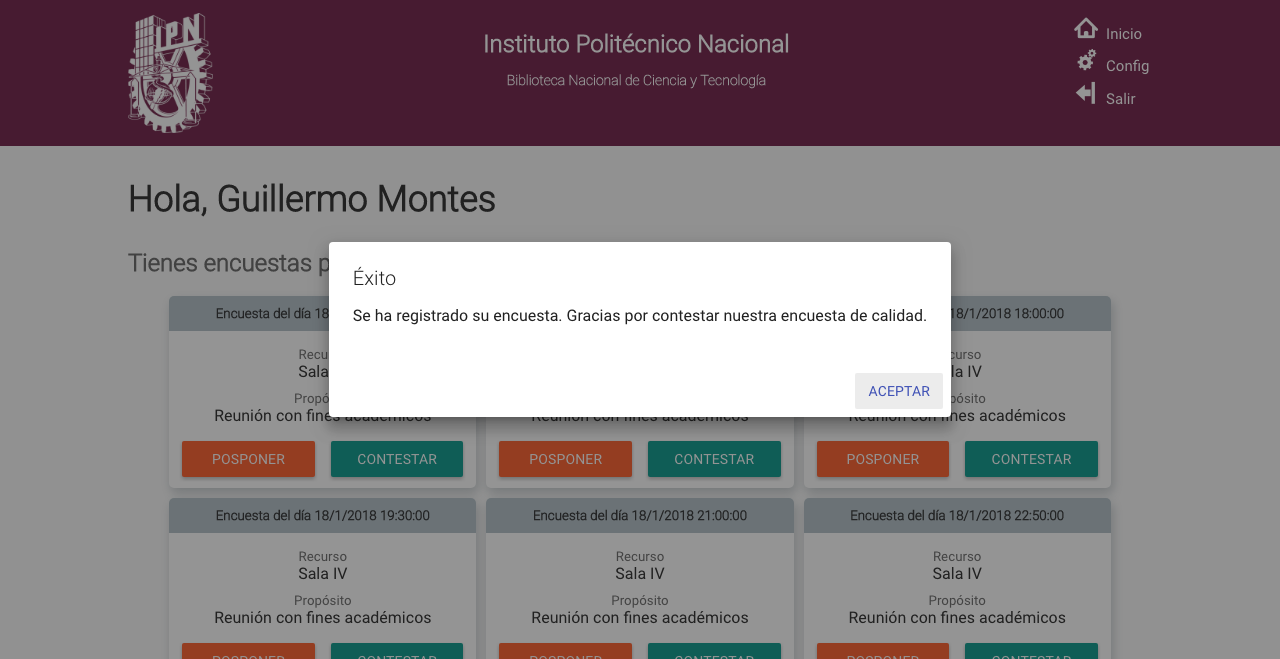
\includegraphics[scale=0.3]{images/Interfaz/MAT-34 Encuesta registrado exitosamente.png}
	\caption{Encuesta registrado exitosamente}
	\end{figure}
\end{enumerate}

  \subsection{ER-01: Cancelar envío de las respuestas de la encuesta}
\begin{enumerate}
	\item Presione el botón \textbf{Cancelar} para continuar en el
  \textit{SUBCUAT-01 Armar interfaz de inicio}.
  \begin{figure}[hbtp]
	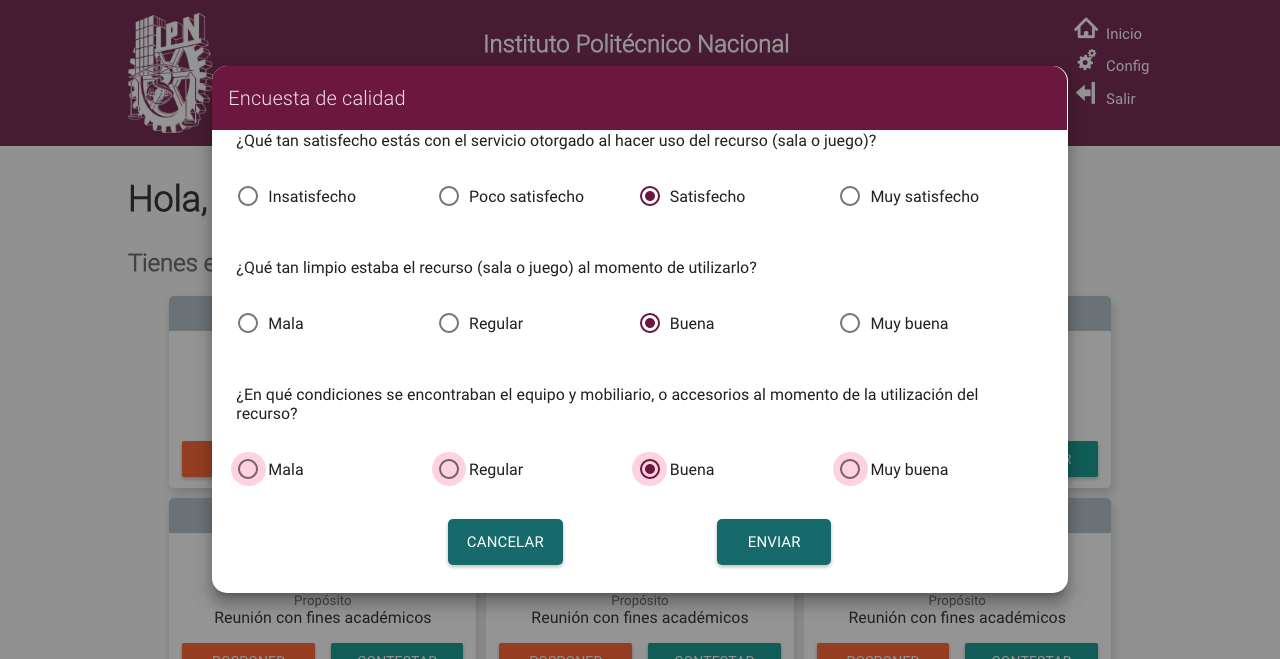
\includegraphics[scale=0.3]{images/Interfaz/Errores Encuesta.png}
	\caption{Cancelar Encuesta}
	\end{figure}
\end{enumerate}

  \subsection{ER-02: Dejar campos incompletos}
\begin{enumerate}
	\item Acepte el mensaje emergente \textbf{MAT-35 Datos incompletos en la encuesta}.
	\item Repita el subpaso 1-A.
	 \begin{figure}[hbtp]
	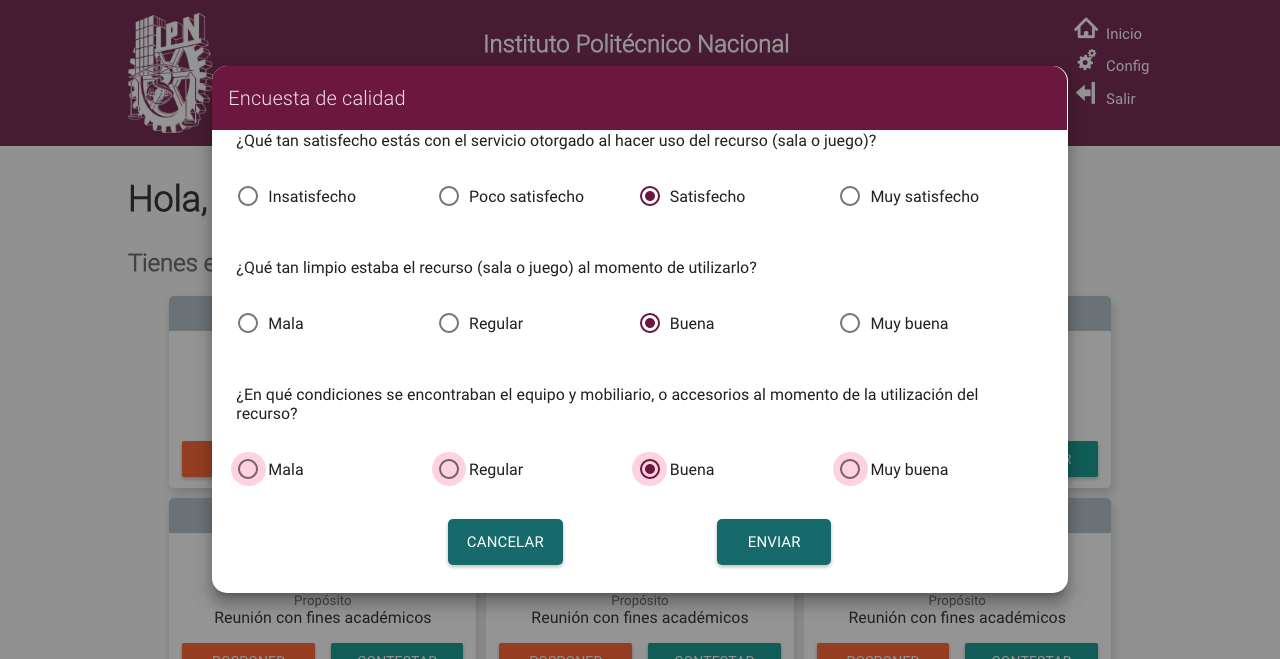
\includegraphics[scale=0.3]{images/Interfaz/Errores Encuesta.png}
	\caption{Campos incompletos encuesta}
	\end{figure}
\end{enumerate}
